\chapter{Revealing Object Interactions with \textsc{PathObjects}}
\chaptermark{Revealing Object Interactions}
\label{c:approach}
This chapter presents \textsc{PathObjects}, an interactive diagraming concept which aims at assisting developers in object-oriented program comprehension.
Section \ref{s:ApproachConcept} describes how our proposed solution helps to bridge the gap of abstraction levels developers face during software engineering.
Section \ref{s:ApproachNotation} presents the basic components of the interactive object communication diagrams that serve this purpose.
With interactivity being an integral part of the concept, \textsc{PathObjects} diagrams also feature a number of interactive components.
They are depicted in Section \ref{s:ApproachInteractivity}.
Finally, Section \ref{s:ApproachLayout} defines aesthetic requirements which should be met by implementations of \textsc{PathObjects}.

\section{Concept}
\label{s:ApproachConcept}
As depicted in Chapter \ref{c:Background}, there are three related problem areas which are tackled in this thesis.
First, there is a huge gap between the abstraction level of the inner workings of computers and the abstraction level of object-oriented source code and design documents.
Moreover, widespread development tools such as symbolic debuggers contribute little to the bridging of this gap.
This is one of the reasons why program comprehension is a tedious and time-consuming task.

Second, dynamic analysis is a fundamental requirement for the analysis and thus for the comprehension of object-oriented programs.
However, traditional approaches suffer from the massive amount of data that arises during program tracing.
Perscheid et al. have proposed step-wise run-time analysis to deal with this problem.
Nevertheless, this approach neither is capable to cover object interactions in its current form, and the verification of its applicability to the visualization of object interactions is still pending.

Third, well-known diagram notations that cover objects states and interactions like those included in the Unified Modeling Language are of static nature.
Mainly for this reason, they seem ill-suited for the use in conjunction with execution traces.
They grow fast, are not capable of covering object state changes over the course of time, and generally do not ease perceivability when being used to visualize scenarios of larger scale, such as those resulting from unit test executions.

As solution to those problems, we propose \textsc{PathObjects}, a concept for the interactive diagraming of object interactions.
The basic idea is to provide developers with an information presentation of object-oriented program behavior at the abstraction level of objects and their interactions.
Thus, we aim at closing the gap between the low-level abstractions of the inner workings of computers, and the high-level abstractions of object-oriented programming languages and design documents.
For that reason, we propose a diagram notation that covers objects, messages, object states, and the roles objects play during message exchanges.
These fundamental diagram elements are described in detail in Section \ref{s:ApproachNotation}.

In order to avoid the waiting time overhead of traditional dynamic analysis tools, we propose to enhance step-wise run-time analysis to make it suitable for the tracing of object interactions.
As shown in Section \ref{s:DiscussionEvaluation}, the immediate provisioning of interactive object communication diagrams can be made possible through this tracing mechanism.
However, this choice entails two consequences.
The first is that execution traces of test cases, or any reproducible program execution for that matter, serve as scenarios for visualization.
Second, it implies interactivity as fundamental technical requirement of the information presentation.
Refinement runs have to be performed to gather information of interest (cf. Section \ref{ss:BackgroundTracing}), and this can only be done in an interactive and iterative process.
Consequently, the information presentation must provide means that allow developers to steer this process.

But there is a further, non-technical reason why interactivity is important.
As pointed out in Section \ref{ss:BackgroundAnalysisProblems}, the usefulness of many dynamic analysis tools is on the one hand limited by the sheer amount of displayed data  but on the other hand constrained to the information that has been collected up front.
However, to maintain perceivability, it is essential to limit the amount of information that is displayed to developers.
An interactive environment is ideal to achieve this purpose.
Developers can be enabled to hide irrelevant information, but they also can request to display information that has neither been displayed nor collected before.
Thus, diagrams can be constructed that cover exactly the relevant amount of information.
Furthermore, execution traces represent data with a chronological ordering.
Instead of displaying the whole chronology at once, interactivity allows developers to jump to specific points of an execution history, and thus to replay a recorded execution.
Again, this drastically reduces the amount of data that is presented to developers simultaneously.

Consequently, we propose a number of interactive components as integral part of \textsc{PathObjects} diagrams.
First, navigational components facilitate exploratory and target-oriented navigation, which means that developers are enabled to explore the temporal and spatial dimensions of execution traces and to search for specific entities of interest.
Second, exploratory components allow developers to explore object states, references, and the underlying source code.
Third, focusing components permit developers to exclude irrelevant objects and messages from the information presentation. 
Finally, information layers allow developers to augment diagrams with use-case specific information.
These four component categories are described in detail in Section \ref{s:ApproachInteractivity}.

\section[Fundamental Diagram Notation]{Fundamental Diagram Notation%
\sectionmark{Diagram Notation}}
\sectionmark{Diagram Notation}
\label{s:ApproachNotation}

\begin{figure}[tb]
	\centering
	
	\begin{subfigure}[b]{1.0\textwidth}
		\centering
        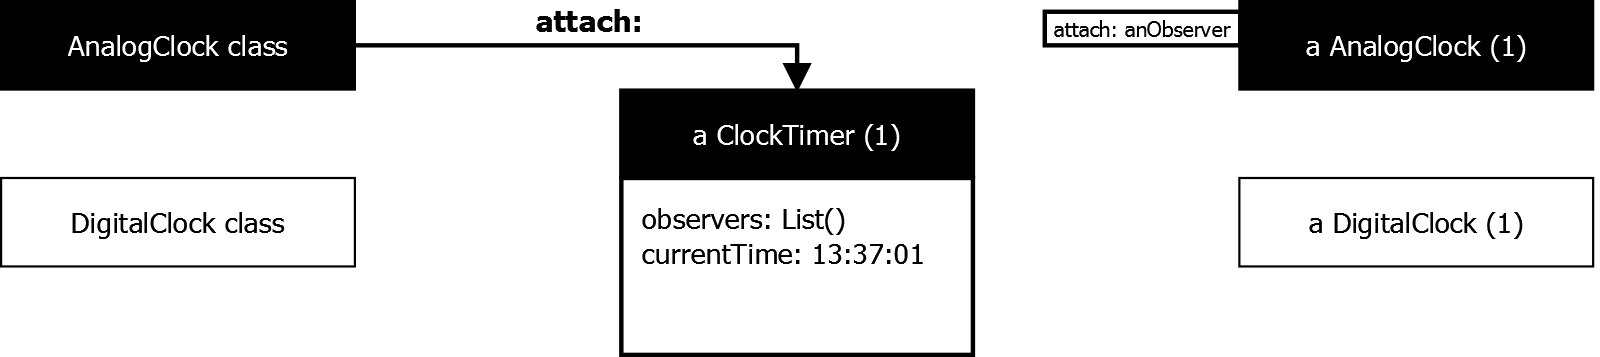
\includegraphics[width=\textwidth]{../images/03-PathObjects-Before}
        \caption[Before the Execution of the Current Message]{}
		\label{fig:ApproachBasicBefore}
	\end{subfigure}
	
	\vspace{1.0cm}
	
	\begin{subfigure}[b]{1.0\textwidth}
		\centering
		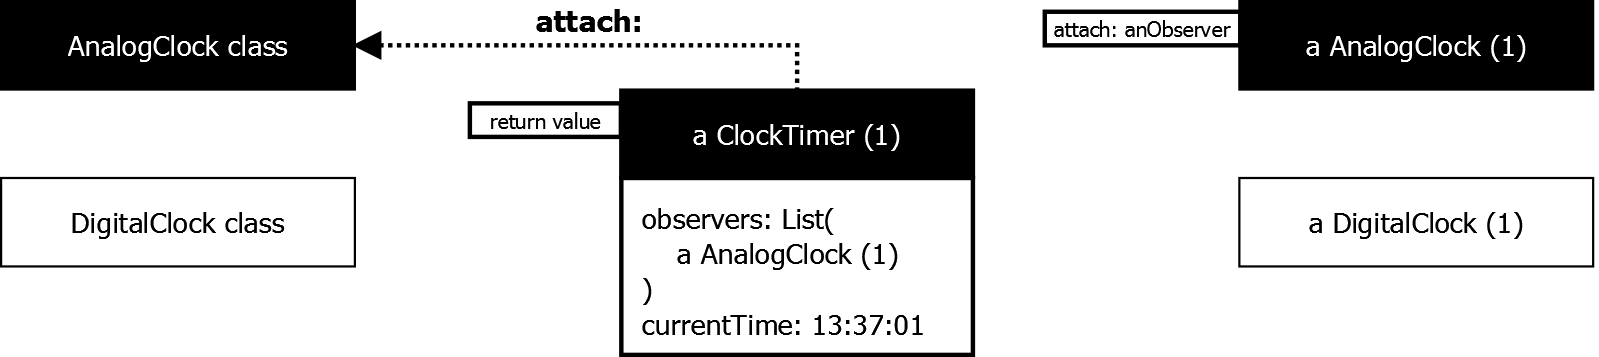
\includegraphics[width=\textwidth]{../images/03-PathObjects-After}
		\caption[After the Execution of the Current Message]{}
		\label{fig:ApproachBasicAfter}
	\end{subfigure}
	
	\caption[Exemplary \textsc{PathObjects} Diagram]{\textsc{PathObjects} diagram of the scenario depicted in Listing \ref{lst:ApproachExample}, (a) before and (b) after the execution of the \inlinecode{attach:} message.}
	\label{fig:ApproachBasic}
\end{figure}

This section describes the fundamental elements of the \textsc{PathObjects} diagram notation.
To ensure a certain degree of recall value, it closely orients on the concepts that are defined by the Unified Modeling Language (cf. Section \ref{s:BackgroundModeling}).
Section \ref{ss:ApproachNotationObjects} shows the representation of objects, which is very similar to communication diagrams.
Section \ref{ss:ApproachNotationMessages} presents the basic illustration of message exchanges, which borrows elements from sequence diagrams.
Section \ref{ss:ApproachNotationRoles} describes role indicators, which are used to mark arguments and return values. 
Finally, Section \ref{ss:ApproachNotationState} presents state indicators, which are comparable to the illustration of object states in UML object diagrams.

All components are illustrated with the help of the example scenario from Section \ref{ss:BackgroundModelingExample}.
Figure \ref{fig:ApproachBasic} covers the process of registering clock instances (observers) at a clock timer instance (subject).
The underlying part of the source code that implements this behavior is depicted in Listing \ref{lst:ApproachExample}.
The analog clock class inherits the \inlinecode{on:} factory method from the observer class.
This method represents the message context in this scenario.
The message that is sent is the \inlinecode{attach:} method, which is implemented by the clock timer class.
The moments before and after the execution of this method serve as examples for the illustration.

\subsection{Objects}
\label{ss:ApproachNotationObjects}
Similar to UML object and communication diagrams, objects are depicted as boxes and can be placed freely on the two-dimensional canvas.
The name of an object is used as caption.
In the case of system-specific singleton objects like classes, no other unique identifier is necessary to ensure distinguishability.
However, this is the case with instances of classes.
Therefore, their name includes a unique integer identifier.
Objects that are somehow involved in the currently displayed message are highlighted through a different background color.
For example, the instances of \inlinecode{ClockTimer} and \inlinecode{AnalogClock} and the analog clock class are involved in the current message in Figure \ref{fig:ApproachBasicBefore}.
Namely, they act as sender, receiver, and argument of the the \inlinecode{attach:}message.
In contrast, the \inlinecode{DigitalClock class} object and the digital clock instance do not play a role in the current computation.

\subsection{Messages}
\label{ss:ApproachNotationMessages}
Messages are represented as directed arrows between objects.
The name of a message is displayed besides the according arrow in plain text.
Just like in the case of UML sequence diagrams, solid arrows indicate message sends (cf. Figure \ref{fig:ApproachBasicBefore}), and dashed arrows indicate message returns (cf. Figure \ref{fig:ApproachBasicAfter}).
The sender and receiver of a message are distinguishable through the direction of the according arrow.
In contrast to sequence diagrams, there is no specific chronological ordering.
Messages that are depicted above a specific message do not necessarily have to occur before it in an execution history.
\textsc{PathObjects} diagrams reveal the chronological relationships only through the element of interactivity (cf. \ref{ss:ApproachInteractiveNavigation}), and usually display only the full details of one message at once.

\begin{smalltalk}[caption={Underlying implementation of the scenario depicted in Figure \ref{fig:ApproachBasic}. The current step of the execution is highlighted.}, label=lst:ApproachExample, escapechar=!]
Observer >> on: aSubject
	| observer |
	observer := self new
		subject: aSubject;
		yourself.
	!\colorbox{YellowGreen}{aSubject attach: observer.}!
	^ observer.

ClockTimer >> attach: anObserver
	observers add: anObserver.
\end{smalltalk}

\subsection{Role Indicators}
\label{ss:ApproachNotationRoles}
Objects that are involved in a message send can play one or more of the four roles sender, receiver, argument, or return value.
The sender and receiver of a message are easily recognizable since they are connected by directed arrows.
However, with message arguments and return values, the case is not as unambiguous.
For that reason, \textsc{PathObjects} diagrams feature indicators for the latter two roles.
For instance, the analog clock instance is an argument of the current message in Figure \ref{fig:ApproachBasicBefore}.
When looking at the according source code of the \inlinecode{attach:} message (cf. Listing \ref{lst:ApproachExample}), it can be seen that the temporary variable name that is used for this part of the selector is \inlinecode{anObserver}.
Since the choice of this name can give important hints about the purpose of an object,
both the part of the selector and the appropriate temporary variable name are displayed as flag alongside the object.

In Figure \ref{fig:ApproachBasicAfter}, a further role indicator is displayed.
Since the diagram now shows a message return, one of the objects has to be the return value, unless the response is a object that is not covered by the trace.
As can be seen in Listing \ref{lst:ApproachExample}, the \inlinecode{attach:} message does not have an explicit return statement.
Consequently, the receiving object itself is the return value, and the corresponding flag is attached to the clock timer instance.

\subsection{State Indicators}
\label{ss:ApproachNotationState}
The information representation of object states is very similar to UML object diagrams.
An additional box is added below the header of objects, and the values of instance variables are displayed within its bounds.
However, there are two significant differences.
First, since object exploration also is an interactive component of \textsc{PathObjects} diagrams (cf. Section \ref{ss:ApproachInteractiveExploration}), the state indicator is only visible for explicitly selected objects.
Second, since the diagrams are interactive rather than static, the state indicators can be used to track object state changes over the course of time.
For instance, Figure \ref{fig:ApproachBasicBefore} depicts the internal state of the clock timer instance before the execution of the \inlinecode{attach:} message.
The state indicator shows that the object has two instance variables, namely an empty list of observers and the current time.
After stepping forward through the execution history, the view changes as depicted in Figure \ref{fig:ApproachBasicAfter}.
Now the diagram shows the state of the object after the execution of the \inlinecode{attach:} message.
Just as the underlying implementation of this message indicates, the analog clock instance now has been added to the list of observers.

\section[Interactive Diagram Components]{Interactive Diagram Components%
\sectionmark{Interactive Components}}
\sectionmark{Interactive Components}
\label{s:ApproachInteractivity}
As depicted in Section \ref{s:ApproachConcept}, interactivity is an integral part of \textsc{PathObjects} diagrams.
Consequently, they provide a number of interactive components which are covered in the following sections.
The components that allow developers to navigate through the temporal and spatial dimensions of diagrams are presented in Section \ref{ss:ApproachInteractiveNavigation}.
The explorative features that can be used to gain insight into the runtime state and the state of the according source code representations are depicted in Section \ref{ss:ApproachInteractiveExploration}.
In order to allow developers to focus on specific entities of interest, \textsc{PathObjects} diagrams feature object and message filters, which are presented in Section \ref{ss:ApproachInteractiveFocusing}.
Finally, information layers can be used to enrich diagrams with use-case specific information, like source code metrics or profiling data.
They are presented in Section \ref{ss:ApproachInteractiveLayers}.

\subsection{Navigation}
\label{ss:ApproachInteractiveNavigation}
Developers have to be allowed to navigate the temporal and spatial dimensions of object interaction diagrams.
For that reason, \textsc{PathObjects} diagrams offer two interactive components, namely the timeline and the mini-map, which allow to examine execution traces in an explorative manner.
The timeline gives an overview of all steps of the execution, or respectively the message sends and returns.
In contrast, the mini-map gives an overview of all objects that occur during the execution, and those that are currently visible in the viewport.

But developers also should be assisted to find specific entities of interest, provided that these entities are already known.
Therefore, a third interactive component facilitates target-oriented navigation, namely the search bar.
It allows developers to find occurrences of classes, message sends, or specific instances of interest.

All three components are described in detail in the following sections.

\subsubsection{Temporal Navigation}
\begin{figure}[tb]
	\centering
	
	\begin{subfigure}[b]{0.45\textwidth}
		\centering
        
\includegraphics[width=\textwidth]{../images/04-ImplTimeline1}
        \caption[Default View]{}
		\label{fig:ApproachTimelineDefault}
	\end{subfigure}
	\quad
	\begin{subfigure}[b]{0.45\textwidth}
		\centering
		
\includegraphics[width=\textwidth]{../images/04-ImplTimeline2}
		\caption[Search Result Highlighting]{}
		\label{fig:ApproachTimelineSearch}
	\end{subfigure}
	\quad
	\begin{subfigure}[b]{0.45\textwidth}
		\centering
		
\includegraphics[width=\textwidth]{../images/04-ImplTimeline3}
		\caption[Differing Metrics Applied to Item Height and Color]{}
		\label{fig:ApproachTimelineMetrics}
	\end{subfigure}
	
	\caption[Variations of the Timeline Component]{Three variations of the timeline component that show the exact same execution history; in each case, the current step is highlighted and the according return point is marked in red.
		a) Default view with mapping of stack depth to item height.
		b) Search result highlighting.
		c) Differing metrics applied to item height and item color.
	}
	\label{fig:ApproachTimeline}
\end{figure}

Developers have to be enabled to navigate through the temporal dimension of execution traces.
On the one hand, stepwise forward and backward navigation should be facilitated.
On the other hand, it also should be possible to jump to specifics points of time in the execution history.
For these reasons, we propose an interactive diagram element, the so-called timeline.

Figure \ref{fig:ApproachTimeline} shows examples of the timeline component.
Each bar represents a step of the execution history, or respectively either a message send or the return from a message send.
The alignment along the horizontal axis corresponds to the chronological order of appearances.
The current step is marked with a blue overlay, and the corresponding send or return step is marked in red.
For instance, the timeline could be used to allow developers to navigate through the execution history by selecting a specific step or by using the keyboard's left and right arrows.

All three examples in Figure \ref{fig:ApproachTimeline} show the exact same execution history at the exact same point of the execution.
Figure \ref{fig:ApproachTimelineDefault} represents the default configuration of the timeline component.
In this case, the height of the single timeline items corresponds to the depth of the call stack.
However, the concept of information layers (cf. Section \ref{ss:ApproachInteractiveLayers}) allows to map arbitrary metrics to this dimension of the diagram.

Figure \ref{fig:ApproachTimelineSearch} shows how search results can be highlighted within the timeline.
In the depicted example, the developer performed a search for occurrences of the \inlinecode{attach:} message.
Two matches are found, whereby each consists of a send and a returns step.
These occurrences correspond to the registration of the analog and digital clock instances at the clock timer.

Figure \ref{fig:ApproachTimelineMetrics} illustrates the usage of information layers in conjunction with the timeline view.
The height of the items now no longer represents the stack depth, but the number of variable accesses in each method.
The item colors indicate the lines of code of each message.
One can see that the current step is the one with by far the most variable accesses.
Furthermore, the visualization indicates that most methods have an acceptable length, with the exception of the method that is currently selected.

\subsubsection{Spatial Navigation}

\begin{figure}[tb]
	\centering
	
	\begin{subfigure}[b]{0.45\textwidth}
		\centering
		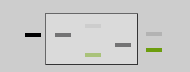
\includegraphics[width=\textwidth]{../images/04-ImplMinimap1}
		\caption[Default View]{}
		\label{fig:ApproachMinimapDefault}
	\end{subfigure}
	\quad
	\begin{subfigure}[b]{0.45\textwidth}
		\centering
		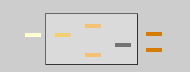
\includegraphics[width=\textwidth]{../images/04-ImplMinimap2}
		\caption[Application of Information Layers]{}
		\label{fig:ApproachMinimapMetric}
	\end{subfigure}
	
	\caption[Variations of the Mini-Map Component]{a) Default configuration of the mini-map component; green represents objects that are involved in the current step, black and gray represent objects occurring in the past or future of the current execution history.
	
	b) \textsc{Fanin} metric applied to the color of objects; black indicates a high number of received messages.}
	\label{fig:ApproachMinimap}
\end{figure}

Contrary to temporal navigation, which allows to explore the chronological dimension of execution traces, developers also have to be enabled to navigate the spatial dimension of interactive communication diagrams.
For that reason, we suggest an interactive miniature representation of diagrams, the so-called mini-map.

The mini-map shows all objects that occur in a trace at a glance and allows to jump to any part of the canvas through mouse interactions.
Furthermore, it depicts which part of the canvas is currently displayed through a miniaturized viewport indicator.
Figure \ref{fig:ApproachMinimapDefault} depicts the default mini-map visualization.
All objects that are involved in the current step, either as sender, receiver, or argument of a message, are marked in green.
Objects that already occurred in the past of the execution history are depicted as black boxes.
Objects that did not occur up to the current step but will occur in future steps are marked in light gray.
Figure \ref{fig:ApproachMinimapMetric} represents an example how information layers can be applied to the mini-map.
In this case, the fan-in metric is mapped to the color of the object representatives.
The heated-object scale indicates few received messages with light colors and the recipience of many messages in dark colors.
One can see that one object, namely the clock timer, receives more messages than any other object in this trace.

\subsubsection{Target-Oriented Navigation}
The spatial and temporal navigation components primarily support explorative approaches.
As opposed to this, developers also should be allowed to navigate to specific entities of interest provided that these entities are already known.
To make this possible, we propose the search bar as third interactive navigation component of our communication diagrams.

The search bar allows developers to find specific entities by reference to their name.
To simplify the process, entities that match a search term are shown and updated as the developer types.
The search functionality supports two different operational modes, namely precise and fuzzy search.
Fuzzy search performs a simple substring matching of the given input, and will return any class instance, class, or message whose name partly or fully matches the given search term.
For instance, this mode makes it possible to find all occurrences of instances of a specific class, by searching for \inlinecode{a ClassName} and omitting the object identifier, which as a matter of fact is part of an object name.
The precise mode, which is enabled as soon as the developer selects an entry from the list of suggested results, allows to search for specific classes, class instances, or messages.
For instance, this allows to search for all occurrences of a specific class.
This would not be possible with fuzzy search alone, since all instances of a class would always also match the search term and would thus lead to a cluttered search result.
As pointed out before, search results are indicated by highlighting timeline items (cf. Figure \ref{fig:ApproachTimelineSearch}).

\subsection{Exploration}
\label{ss:ApproachInteractiveExploration}
Developers have to be enabled to explore the state of the system under observation and to reenact how it changes over the course of time.
For that reason, \textsc{PathObjects} provides two interactive components.
First, state exploration allows to inspect the internal state of objects.
Second, reference exploration allows developers to track the outbound object pointers of specific objects.
Thus, it is possible to reenact how an object obtains and releases references to other objects.
Furthermore, not only the runtime state of the system under observation is relevant, but also the state of the underlying implementation.
Consequently, \textsc{PathObjects} diagrams also keep connections to the source code of the investigated system, and allow developers to explore the according implementations of messages and their senders.
All three components are depicted in the following sections.

\subsubsection{State Exploration}
To allow developers to understand the reasons for the behavior of a system, it is important to give them an insight into the internal state of said system, or respectively of its objects.
For that reason, we propose state exploration as important interactive component of \textsc{PathObjects} diagrams.

State exploration enables developers to monitor the internal state of specific objects over the course of time.
As long as state exploration is enabled for an object, a state indicator is expanded below the object header (cf. Section \ref{ss:ApproachNotationState}).
This means that the values of all instance variables are shown, and complex referenced objects can be explored recursively.
Through automated executions of refinement runs (cf. Section \ref{ss:BackgroundTracing}), the state can be updated whenever the developer steps to a different point of the execution history.

State exploration is not only available for senders and receivers of messages, but also for all arguments and return values.
However, objects that occur in the latter two roles only show up on the canvas if they are either a message sender or receiver elsewhere in an execution history. 
In order to allow for the state exploration of those objects where this is not the case, \textsc{PathObjects} diagrams also feature an external state indicator that is not tied to specific objects.

\subsubsection{Reference Exploration}
As second explorative component, we propose reference exploration, which allows developers to chase outbound pointers of specific objects.
The mechanism works similar to the state exploration described above.
Developers can toggle reference exploration on a per-object basis.
When enabling exploration, the developer is prompted to select a color.
This selection will then be used as background color of all referenced objects.
The current outbound pointers are collected when stepping through the execution history, and the background colors of referenced objects are updated accordingly.
This allows developers to get an insight which other objects a specific one references, when these references are gained, and when they are released.

\subsubsection{Source Code Exploration}
The essential goal during program comprehension is to map the behavior of a software system to its source code representation.
For that reason, we propose source code exploration as third interactive component.
With the help of this component, \textsc{PathObjects} diagrams stay connected to the underlying source code of the system under observation at all times during the exploration of an execution trace.
The context in which a method is called - the implementation of the calling method - and the implementation of the called method itself can be explored through a source browser pop-up.

\subsection{Focusing}
\label{ss:ApproachInteractiveFocusing}
In order to allow developers to focus on specific entities of interest, we propose interactive components for the filtering of irrelevant objects and messages.
Both mechanisms are presented in the following.

\subsubsection{Message Filter}

\begin{figure}[tb]
	\centering
	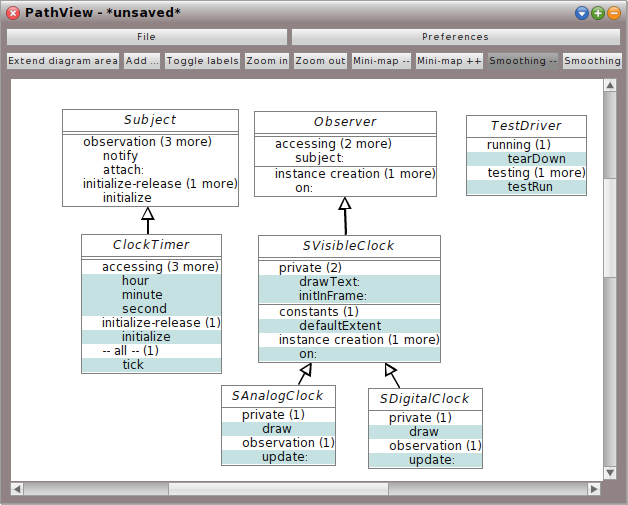
\includegraphics[width=0.7\textwidth]{../images/04-ImplMessageFilter}
	\caption[Exemplary Static Structure Visualization]{Exemplary static structure visualization as provided by \textsc{PathView}.}
	\label{fig:ImplementationFocusingMessages}
\end{figure}

To allow developers to remove irrelevant messages from the canvas, we propose to create views of the static structure of entities that occur in an execution trace.
With the aid of this view, messages that should be displayed or removed can be selected or respectively deselected.
The \textsc{PathTools} suite already provides similar tool, namely \textsc{PathView} \cite{perscheid_test-driven_2013}.
The primary purpose of this tool is to generate UML class diagrams from execution traces.

Figure \ref{fig:ImplementationFocusingMessages} shows how such a message filter could be realized with the help of \textsc{PathView}.
It shows all classes that are represented by object instances in the current trace, namely the abstract and concrete \inlinecode{Subject} and \inlinecode{Observer} classes as well as a class from the test environment (\inlinecode{TestDriver}).
Thereby, only those methods that occur in a trace are displayed.
With the help of this information presentation, single methods can be selected and deselected.
Whenever the developer changes a selection, the \textsc{PathObjects} visualization can be updated, and messages that represent those methods can be removed from or re-added to the visualization.
In the depicted example, all methods are selected, except those implemented by the abstract \inlinecode{Subject} and \inlinecode{Observer} classes.

\subsubsection{Object Filter}
To allow developers to focus on one or more specific objects of interest, we propose the object filter as second filtering component.
For instance, if one chooses to focus on the digital clock instance through the object filter, the \inlinecode{SAnalogClock} class object and the instance of \inlinecode{SAnalogClock} will be removed from the canvas.
In addition, all messages that do not involve the selected object are removed from the timeline.
All other objects remain on the canvas, since they exchange messages with the selected object at some point of the execution history.

Developers then can broaden the focus area through the selection of further objects of interest.
For example, the clock timer instance can be added to the selection, which will bring back the analog clock components and the according messages to the canvas.

Since the selection of a small set of relevant objects usually reduces the number of displayed objects drastically, objects can be rearranged automatically with every change of the current selection.
Thus, the information presentation can be compacted for perceivability purposes.

\subsection{Information Layers}
\label{ss:ApproachInteractiveLayers}
Program comprehension usually does not end in itself but rather serves a specific purpose.
Consequently, the situations in which developers try to build an understanding of a software system are manifold.
Furthermore, different purposes require different additional information that can assist developers in specific situations.

For instance, if a developer wants to fix a defect, information such as recent changes that have been made to the system might be of interest.
Furthermore, one might want to display root cause probabilities along with methods.
In contrast, if the goal is a general refactoring to improve the overall code quality, one might be interested in metrics like lines of code or cyclomatic complexity.
The elimination of performance bottlenecks constitutes another common scenario.
In this case, developers most likely are interested in runtime profiling data.
When using conventional development tools, all this information usually has to be collected with different tools, and has to be integrated into the current context by developers manually.

At the same time, many dimensions of \textsc{PathObjects} diagrams are unused in the sense that they do not transport any semantic information.
The size of object nodes, the width of message connectors, the color and extent of timeline items, or the size and color of fonts constitute examples.
In addition, some facts are encoded redundantly.
For instance, objects that are somehow involved in the current step of the execution history are highlighted.
However, senders and receivers of messages are also clearly recognizable through  message connectors, and arguments and return values are flagged with role indicators.
As a consequence, this dimension could also be used to visualize additional information that would otherwise not be present in a diagram.

For these reasons, we propose the concept of information layers, which allow developers to project arbitrary metrics to various dimensions of \textsc{PathObjects} diagrams.
Thereby, metrics can provide data for messages and objects.
Table \ref{t:ApproachLayers} lists exemplary metrics that are also provided by our prototypical implementation of \textsc{PathObjects} for Squeak/Smalltalk (cf. Chapter \ref{c:implementation}).
The dimensions that are supported for the visualization of a metric are dependent on the kind of data it provides.
Therefore, Table \ref{t:ApproachLayers} relates the metrics to the diagram dimensions they could be mapped to.
For instance, the information about recent method changes could be projected to the color of timeline items or the width of message connectors.
Similarly, the fan-in metric which yields data about objects could be mapped to the color of object nodes or their color on the mini-map.

Developers can add as many information layers to a \textsc{PathObjects} diagram as they want.
The number of layer combinations and their expressiveness is only limited by the number of diagram dimensions that are available.
Thus, developers are enabled to integrate a diversity of information into the scenarios that are used to build an understanding of the system at hand.
The requirement to collect information from various tools manually can be eliminated for many use-cases.
Consequently, the concept of information layers has the potential to reduce the time spent on program comprehension even further.

\begin{table}[tb]
	\centering
	\footnotesize
	\begin{subtable}[t]{0.45\textwidth}
		\begin{tabular}{ll}
		\toprule[1.2pt]
		Message Metrics		& Dimensions 			\\
		\midrule
		Complexity			& Edge Color 			\\
		Last Change			& Edge Width			\\
		Lines of Code		& Timeline Item Color	\\
		Runtime Profiling	& Timeline Item Height	\\
		Stack Size			&						\\
		Variable Accesses	&						\\
		\bottomrule[1.2pt]
		\end{tabular}
		\caption[Message Metrics]{}
	\end{subtable}
	\qquad
	\begin{subtable}[t]{0.45\textwidth}
		\begin{tabular}{ll}
		\toprule[1.2pt]
		Object Metrics		& Dimensions 			\\
		\midrule
		\textsc{Fanin}		& Mini-Map Color		\\
		\textsc{Fanout}		& Object Color			\\
		\textsc{Faninout}	& Object Height			\\
		\hphantom{Runtime Profiling}	& Object Width			\\
							& \hphantom{Timeline Item Height} \\
							& \\
		\bottomrule[1.2pt]
		\end{tabular}
		\caption[Object Metrics]{}
	\end{subtable}
	\caption[Information Layers: Possible Metrics and Diagram Dimensions]{Possible (a) message and (b) object metrics that could be used as data source for information layers, together with the diagram dimensions they could be mapped to.}
	\label{t:ApproachLayers}
\end{table}


\section[Diagram Layout and Aesthetics]{Diagram Layout and Aesthetics%
\sectionmark{Diagram Aesthetics}}
\sectionmark{Diagram Aesthetics}
\label{s:ApproachLayout}
When considering the intended usage of \textsc{PathObjects} diagrams, it becomes evident that the automatic computation of diagram layouts is an essential feature of potential implementations of the concept.
The primary purpose is to provide immediate information presentations of selected test cases.
If developers would have to arrange elements in those diagrams manually, a time-consuming task would be introduced by a tool that aims at reducing the time share of another activity, namely program comprehension.

For that reason, it is important do define the aesthetic criteria such automatically generated layouts should adhere to.
Since \textsc{PathObjects} diagrams display graph structures, the research on graph drawing aesthetics can be incorporated.
Graph drawing is a research area with a long history of its own, and there is broad consent about the aesthetic properties that should be aimed at in order to maximize perceivability \cite{battista_graph_1998, kaufmann_drawing_2001, diehl_software_2007}.
Consequently, it stands to reason that these criteria should also be applied to our interactive object communication diagrams.

However, most of those drawing optimization criteria are NP-hard computational problems for tree structures \cite{battista_graph_1998}.
And since the graphs that should be presented through \textsc{PathObjects} diagrams are call trees, this raises the question if the immediate character of the underlying tracing approach can be maintained.
For that reason, a runtime performance evaluation of the diagram construction is presented in Section \ref{s:DiscussionPerformance}.

We propose the following seven aesthetic criteria from the domain of graph drawing as requirements for the layout of \textsc{PathObjects} diagrams:

\paragraph{Crossing Minimization} User studies suggest that the most important aesthetic criterion is the minimization of edge crossings \cite{purchase_effective_2000, purchase_graph_2004, purchase_graph_2010}.
The more edges cross each other, the harder it becomes for the human eye to keep track of the nodes that are connected by an edge.
Graph drawings that do not entail edge crossings are called planar, and are regarded as the best-case scenario.
But although planar graph drawing algorithms are comparatively simple, the excessive optimization of drawings in these premises will most likely interfere with other aesthetic criteria.

\paragraph{Bend Minimization} Bends make it harder for the human eye to follow the route of an edge.
Consequently, both the maximum number of bends on a single edge as well as the total number of bends on all edges should be as low as possible.
Furthermore, the variance of the number of bends on edges should be minimized.
However, recent studies suggest that continuity is more important than the number of bends \cite{diehl_software_2007}.

\paragraph{Length Minimization} Similar to crossings and bends, increasing edge lengths make it increasingly difficult for the viewer of a graph drawing to follow their paths.
Therefore, both the length of the longest edge and the total edge length should be minimized.
In addition, some authors state that the overall variance of lengths should be minimized in order to provide uniform edge lengths \cite{battista_graph_1998, kaufmann_drawing_2001}.

\paragraph{Area Minimization} The minimization of the area a diagram takes up is especially important when it cannot be scaled down arbitrarily.
This is the case with \textsc{PathObjects} diagrams, since textual information associated with nodes and edges has to stay above perceptive thresholds and may not overlap.
Furthermore, the efficient utilization of screen space is important.
Although our interactive information presentation offers scrolling functionality and thus allows diagram extents to exceed the viewport, scrolling interferes with reading the diagram and consequently complicates the assimilation of information.

\paragraph{Symmetry} Nodes should be distributed evenly on the canvas and thus should form a homogeneous density.
Furthermore, if the underlying graph structure features symmetries, these symmetries should also be reflected by the graph drawing.

\paragraph{Clustering} Interconnected parts of a graph should be drawn distinguishable from other so-called clusters.
In our case, connections are established through message exchanges, and objects or respectively nodes are connected stronger if they exchange more messages among each other than with other objects.
In addition, the edges between members of the same cluster should be shorter than edges that connect nodes from different clusters.

\paragraph{Orthogonality} Some authors state that fixing nodes and edges to an orthogonal grid improves the understandability of graph drawings \cite{sugiyama_methods_1981, batini_what_1985}.
And although Purchase et al. could not find significant evidence for this claim in a user study \cite{purchase_which_1997}, the majority of participants that were confronted with different variations of UML collaboration diagrams in another study nevertheless favored this edge routing strategy over other approaches \cite{purchase_graph_2004}.
